\documentclass[11pt, a4paper]{article}
\usepackage[margin=1in]{geometry}
\usepackage{graphicx}
\usepackage{booktabs}
\usepackage{amsmath}
\usepackage{hyperref}
\usepackage{float}
\usepackage{enumitem}
\usepackage{caption}
\usepackage[T1]{fontenc}

\title{\textbf{GBDT vs MLP on the Bank Marketing Dataset}\\[0.3em]
\large Advanced Machine Learning --- Homework 2}
\author{}
\date{}

\begin{document}
\maketitle
\noindent\textbf{Repository:} \url{https://github.com/yumozi/aml-hw2}

% =========================================================================
\section{Introduction}
% =========================================================================

This report compares Gradient Boosted Decision Trees (GBDT) and Multi-Layer
Perceptrons (MLP) on a binary classification task: predicting whether a client
of a Portuguese bank will subscribe to a term deposit after a phone-based
marketing campaign.

The \textbf{Bank Marketing} dataset comes in two versions: an extended version
with 20 input features and a classic version with 17 features (16 inputs + 1
target). We used the classic file (\texttt{bank\text{-}full.csv}) since
detailed descriptions are only provided for the 17-feature version. It contains
45,211 records spanning client demographics, financial indicators, and campaign
attributes. The target is heavily imbalanced: only 11.7\% subscribed (``yes'')
vs.\ 88.3\% (``no''). This controlled experiment---same data, splits, and
evaluation---enables direct comparison of how each model family learns.

% =========================================================================
\section{Methods}
% =========================================================================

\subsection{Data Preparation}

\paragraph{Missing values.}
No nulls exist, but several categorical features use \texttt{"unknown"} as a
placeholder. We considered: (1)~keeping ``unknown'' as its own category,
(2)~imputing with mode, (3)~dropping affected rows (${\sim}25\%$ loss). We
chose option~1 because ``unknown'' itself carries signal---e.g., clients
reached via an unknown contact method came disproportionately from older
campaigns with lower subscription rates.

\paragraph{Feature engineering.}
Three derived features were added:
\begin{itemize}[nosep]
    \item \texttt{was\_contacted\_before}: binary flag from \texttt{pdays}
          ($1$ if previously contacted, $0$ otherwise). 82\% of clients had
          no prior contact.
    \item \texttt{age\_group}: age binned into five groups (young, mid, senior,
          elder, retired).
    \item \texttt{balance\_positive}: binary flag for positive account balance.
\end{itemize}

\paragraph{Duration removal.}
The \texttt{duration} feature was dropped---while highly predictive, it is only
known \emph{after} a call ends and cannot be used for realistic prediction.

\paragraph{Encoding.}
We chose \textbf{one-hot encoding with \texttt{drop\_first=True}} over label
encoding to avoid implying ordinal relationships that could mislead MLP
training, yielding 47 input features.

\paragraph{Train / Validation / Test split.}
A stratified 70\,/\,15\,/\,15 split yielded 31,647 training, 6,782 validation,
and 6,782 test samples. Stratification preserved the ${\sim}11.7\%$ positive
rate across all three sets.

\paragraph{Feature scaling.}
A \texttt{StandardScaler} was \textbf{fit on training data only} and applied to
validation/test sets (no data leakage). Scaling is essential for MLP: neurons
compute weighted sums, so features on different scales (e.g., \texttt{balance}
up to 102,127 vs.\ binary flags) elongate the loss surface, causing unstable
gradients. Standardization (mean$=0$, std$=1$) makes the landscape isotropic.
Trees split on thresholds invariant to monotonic transformations, so scaling is
unnecessary for GBDT.

\begin{figure}[H]
    \centering
    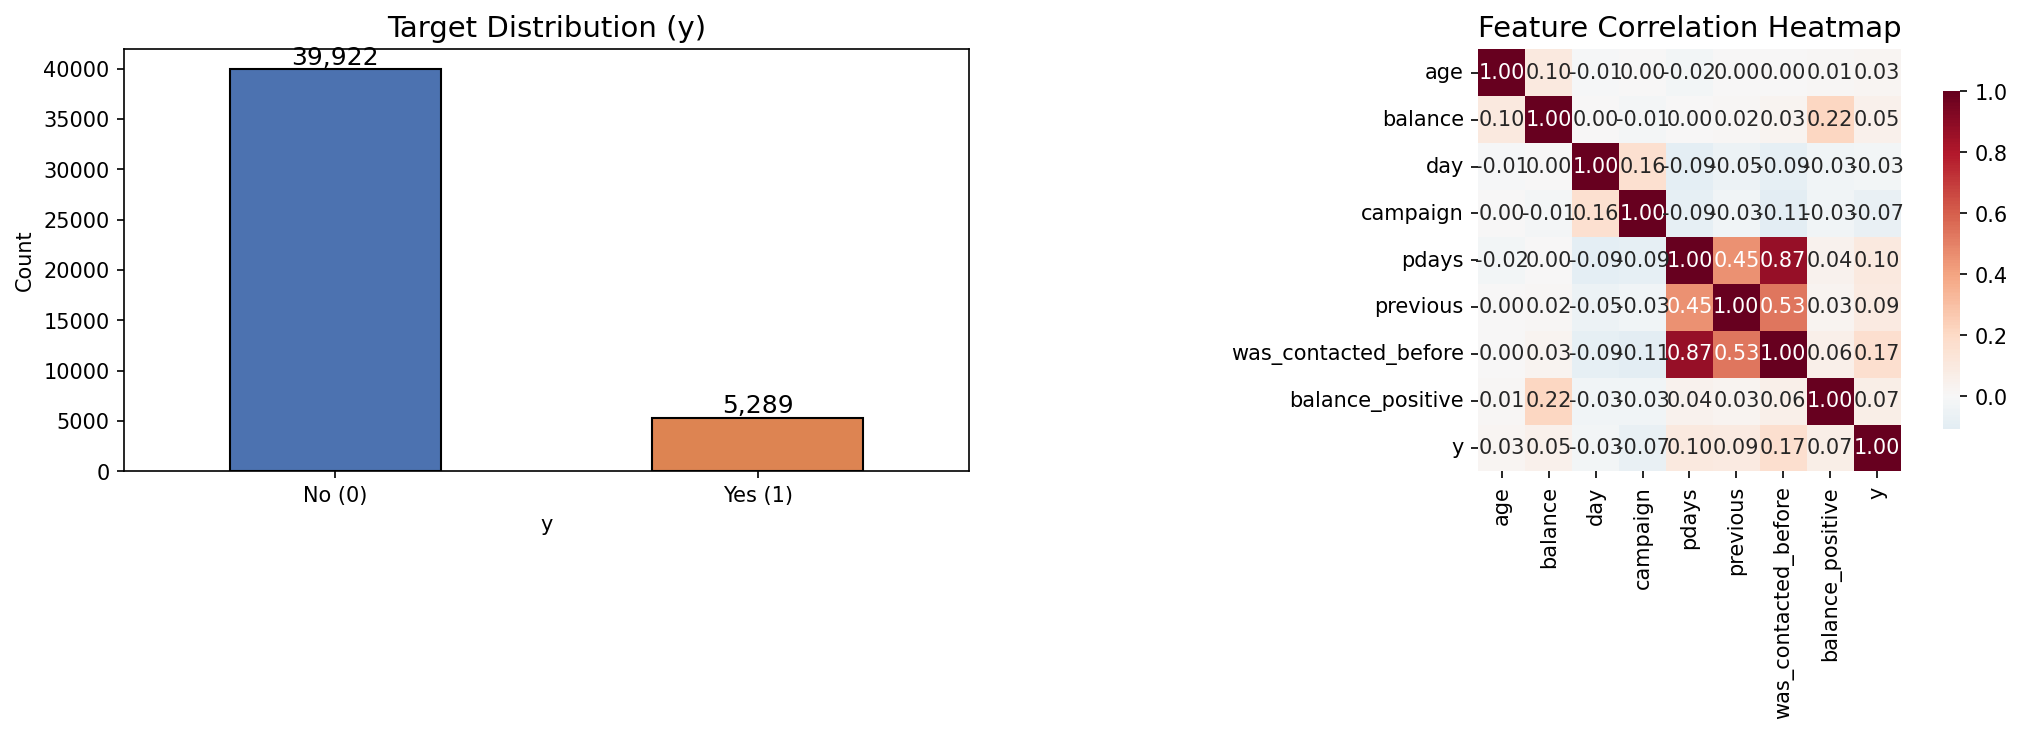
\includegraphics[width=0.75\textwidth]{fig_data_preparation.png}
    \caption{Left: class distribution showing 88:12 imbalance.
             Right: Pearson correlation heatmap of numeric features with the
             target. Most individual correlations are weak ($|r| < 0.15$),
             motivating non-linear models.}
    \label{fig:data_prep}
\end{figure}

% =========================================================================
\subsection{GBDT Implementation (XGBoost)}

We used \texttt{XGBClassifier} from the \texttt{xgboost} library. To address
class imbalance, we set
\texttt{scale\_pos\_weight} $= N_{\text{neg}} / N_{\text{pos}} \approx 7.5$,
which up-weights the minority class in the loss function---analogous to cost-sensitive
learning.

\paragraph{Baseline.}
The initial model used \texttt{learning\_rate=0.1}, \texttt{n\_estimators=500},
\texttt{max\_depth=5}, \texttt{subsample=0.8}. It achieved validation
F1\,$=$\,0.45 for the positive class and trained in under 1 second.
The training-vs-validation loss curve (Figure~\ref{fig:xgb_loss}) showed the
model was still improving at round 490, with a train--val loss gap of
${\sim}0.09$---indicating mild overfitting at most.

\begin{figure}[H]
    \centering
    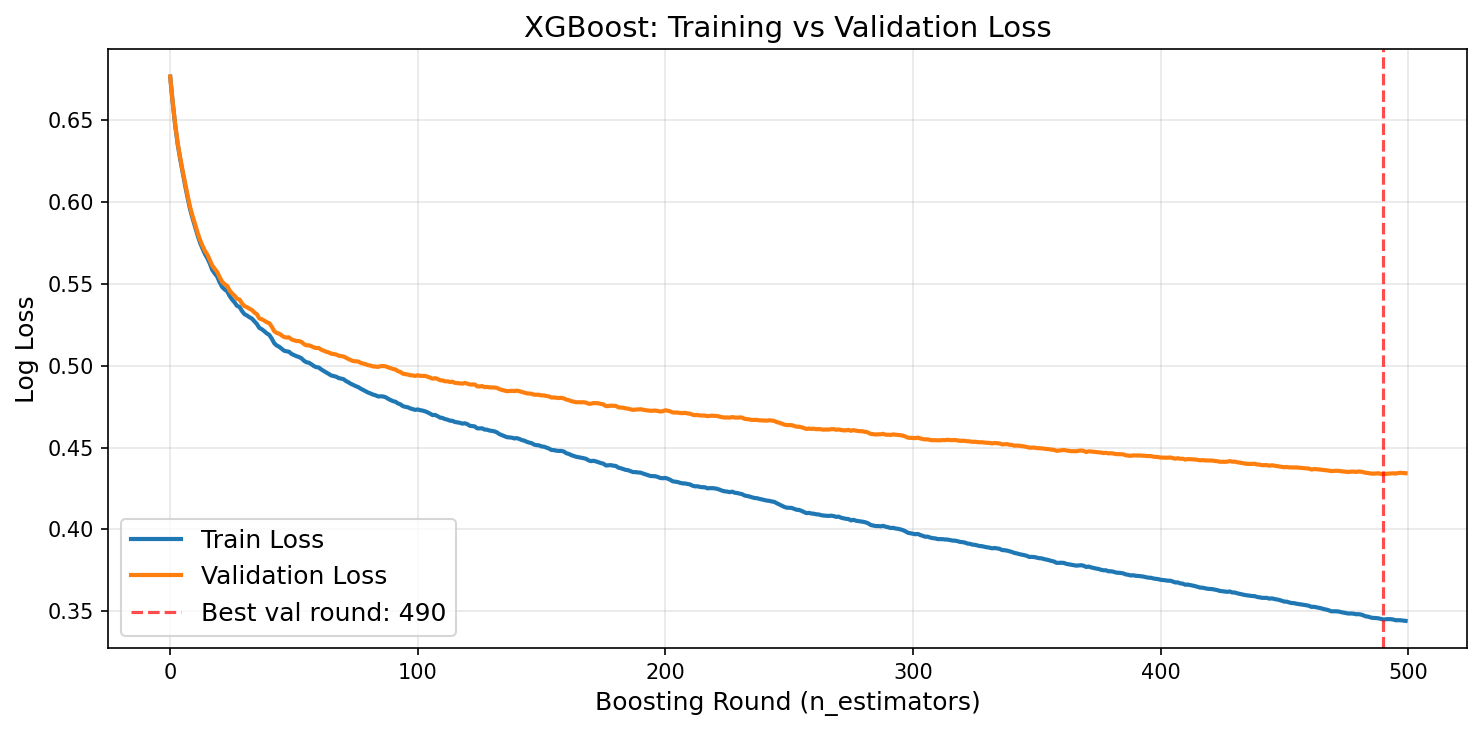
\includegraphics[width=0.65\textwidth]{fig_xgb_loss_curve.png}
    \caption{XGBoost baseline: training vs.\ validation log-loss over 500
             boosting rounds. The red dashed line marks the round with minimum
             validation loss.}
    \label{fig:xgb_loss}
\end{figure}

\paragraph{Learning rate study.}
We compared three learning rates (0.01, 0.1, 0.3) with 500 trees each
(Figure~\ref{fig:xgb_lr}):

\begin{table}[H]
\centering
\begin{tabular}{cccc}
\toprule
Learning Rate & Val Accuracy & Val F1 & Best Round \\
\midrule
0.01 & 0.806 & 0.437 & 499 (still improving) \\
0.10 & 0.830 & 0.450 & 490 \\
0.30 & 0.842 & 0.418 & 490 \\
\bottomrule
\end{tabular}
\caption{Effect of learning rate on XGBoost validation performance.}
\end{table}

A low rate (0.01) converges slowly and needs more trees; a high rate (0.3)
reaches lower loss but sacrifices F1---the model becomes more conservative on
positive predictions, favoring raw accuracy over recall. The rate 0.1 offered
the best F1 trade-off.

\begin{figure}[H]
    \centering
    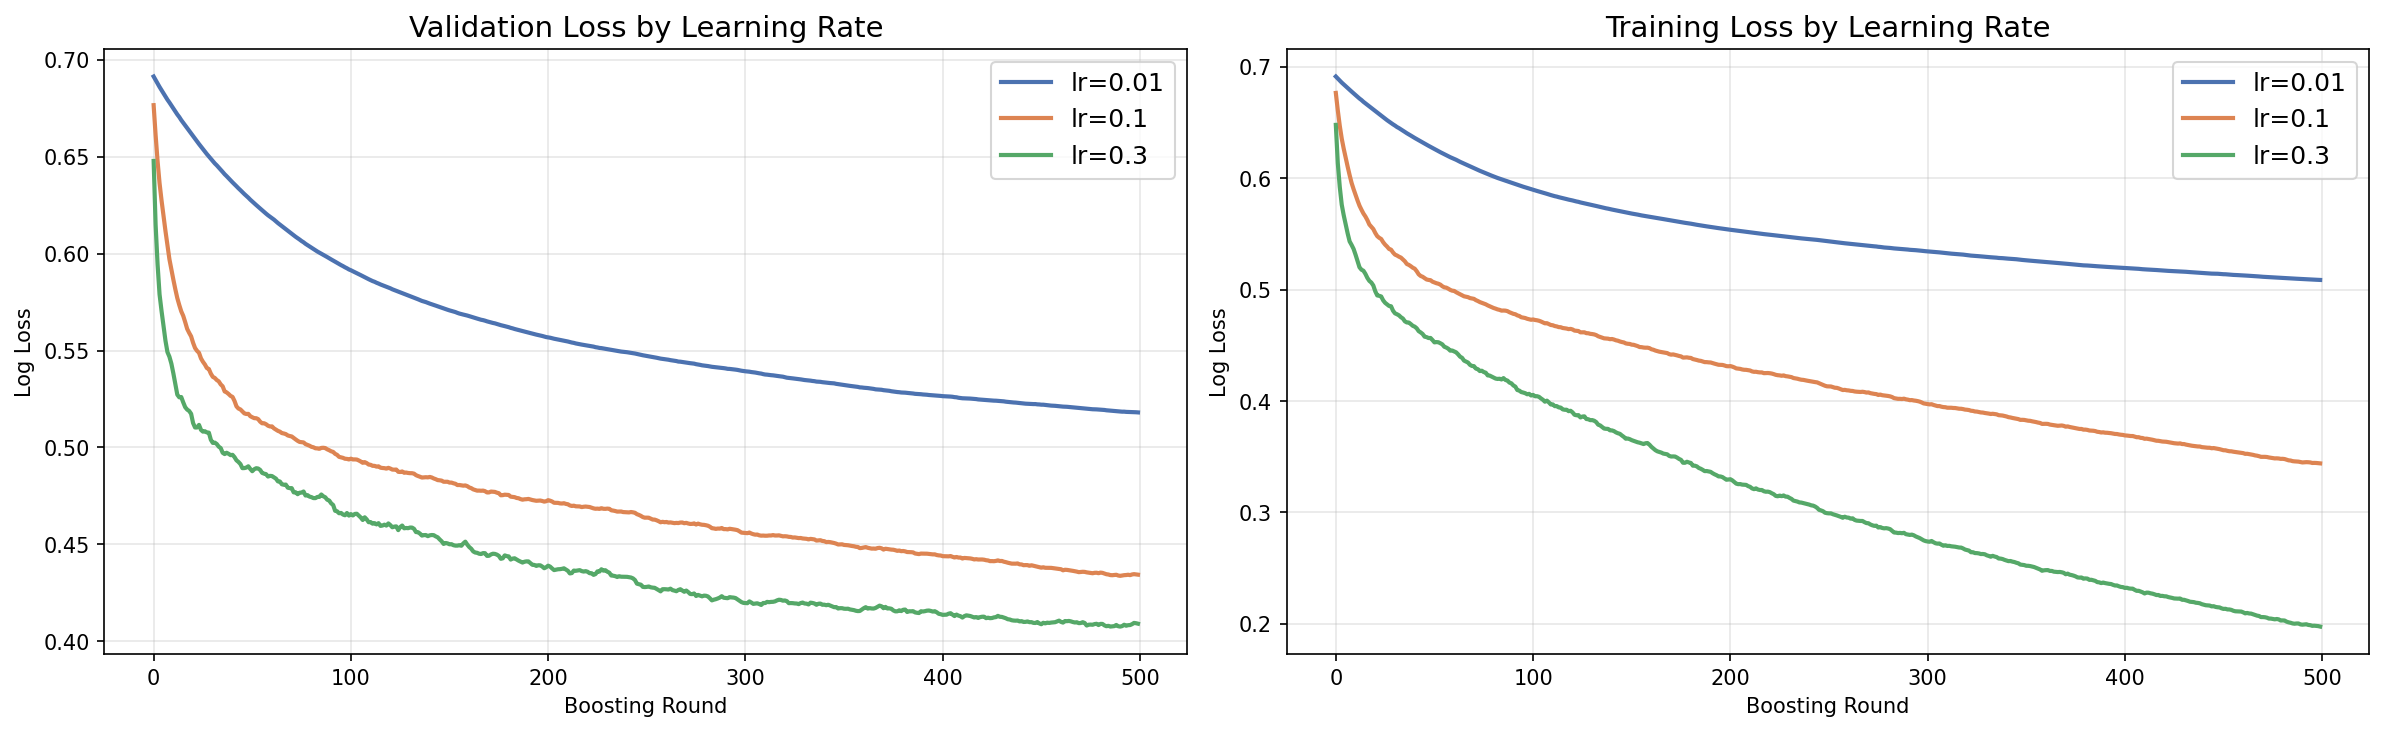
\includegraphics[width=0.75\textwidth]{fig_xgb_learning_rate.png}
    \caption{Validation loss (left) and training loss (right) for three
             learning rates. Lower rates converge more slowly but generalize
             comparably; higher rates risk overfitting earlier.}
    \label{fig:xgb_lr}
\end{figure}

\paragraph{Hyperparameter tuning.}
\texttt{RandomizedSearchCV} explored 30 combinations over
\texttt{learning\_rate}, \texttt{n\_estimators}, \texttt{max\_depth},
\texttt{subsample}, \texttt{reg\_alpha}, and \texttt{reg\_lambda}, using 3-fold
CV with F1 scoring. The best configuration was:
\texttt{lr=0.05, n\_estimators=200, max\_depth=7, subsample=0.7,
reg\_lambda=2.0} (CV F1\,$=$\,0.446).

The tuned model achieved validation precision\,$=$\,0.37, recall\,$=$\,0.63,
F1\,$=$\,0.47---a modest improvement over the baseline, confirming that GBDT
is robust to hyperparameter choices on this dataset.

\begin{figure}[H]
    \centering
    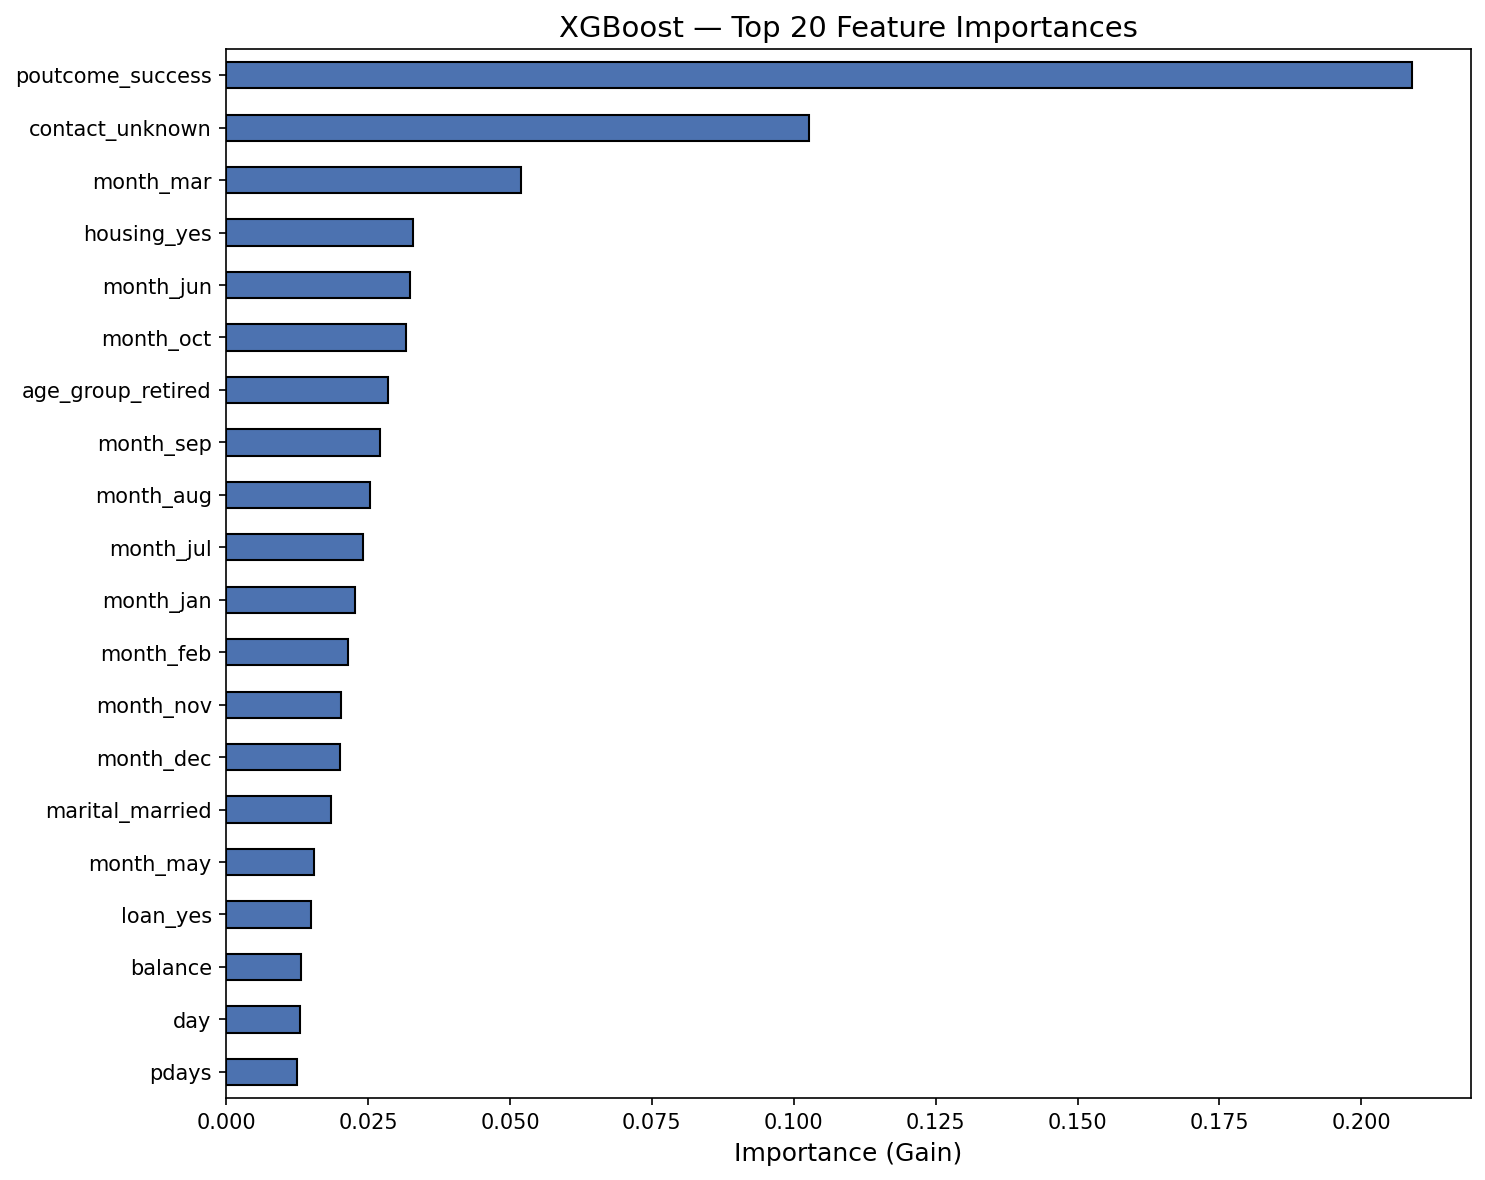
\includegraphics[width=0.6\textwidth]{fig_xgb_feature_importance.png}
    \caption{Top 20 feature importances from the tuned XGBoost model. Previous
             campaign outcome (\texttt{poutcome}), contact method, campaign
             month, and account balance dominate.}
    \label{fig:xgb_importance}
\end{figure}

% =========================================================================
\subsection{MLP Implementation}

We used \texttt{MLPClassifier} from scikit-learn with standardized features.

\paragraph{The class imbalance problem.}
Our first MLP (128 neurons, relu, lr\,$=$\,0.001) converged in only
\textbf{34 iterations} with a validation accuracy of 0.90---but recall for
``Yes'' was just 0.24 and F1 was 0.34. The validation score plateaued at
${\sim}0.9$ from the first iteration because the model immediately learned to
predict ``No'' for nearly everything, achieving 88\% accuracy trivially.

Unlike XGBoost, scikit-learn's \texttt{MLPClassifier} has no
\texttt{class\_weight} parameter. We addressed this by \textbf{oversampling the
minority class}: we randomly resampled the positive class (with replacement) to
match the majority, creating a balanced training set of 55,890 samples (50/50
split). After oversampling, training extended to 235 iterations with meaningful
loss descent, and recall for ``Yes'' improved from 0.24 to 0.48.

\begin{figure}[H]
    \centering
    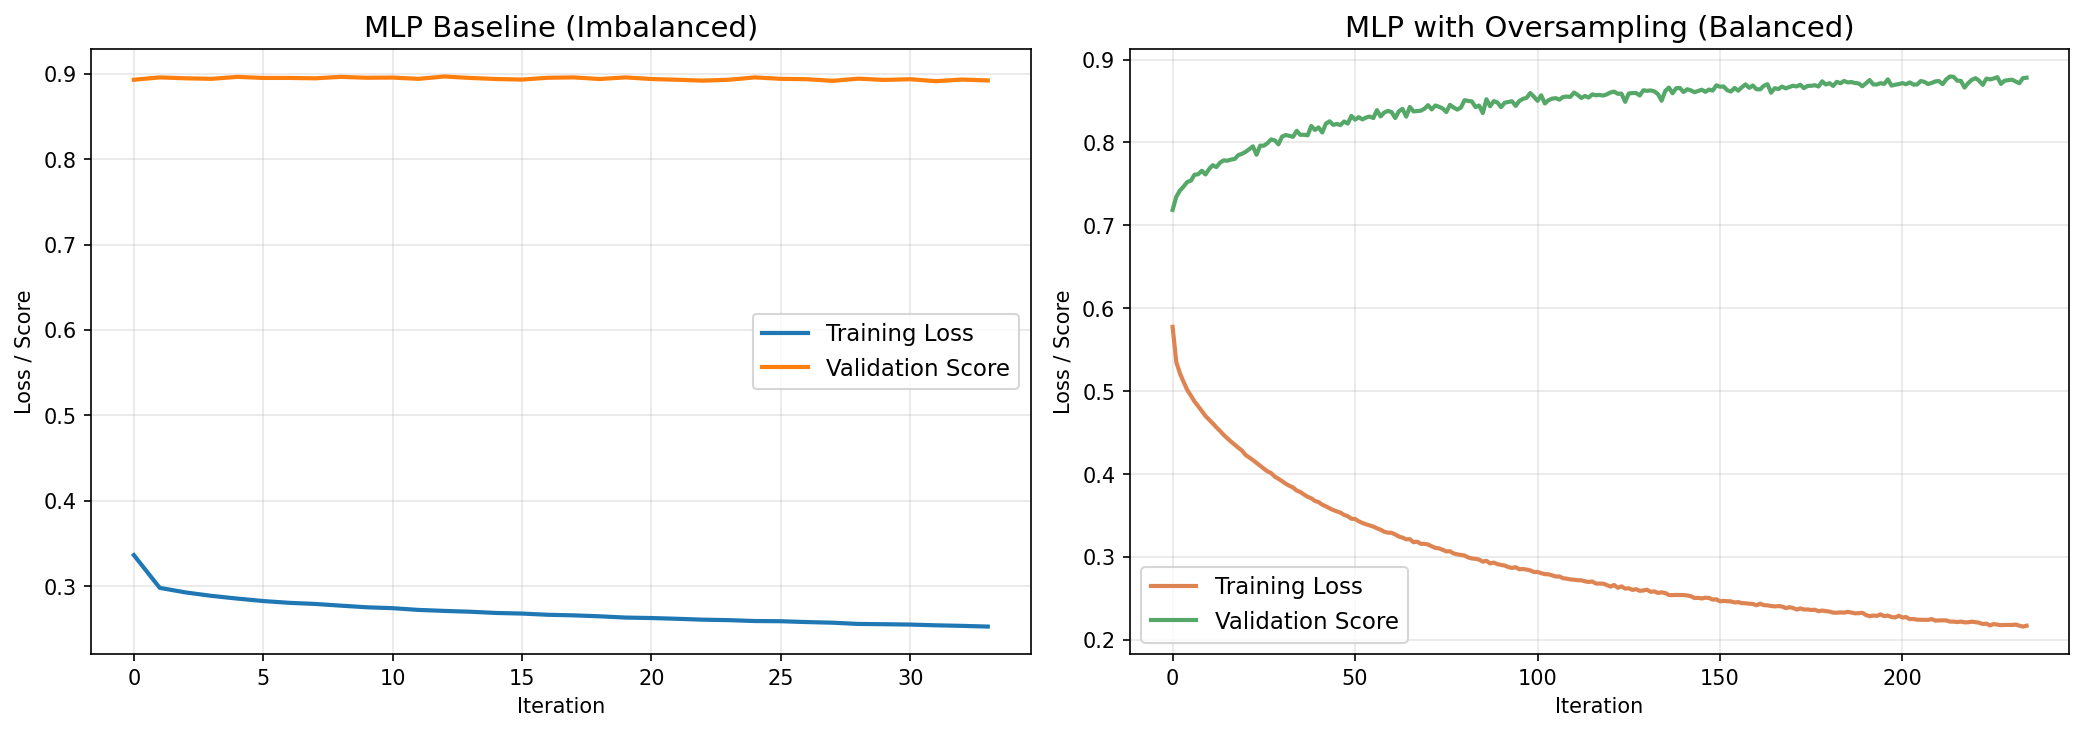
\includegraphics[width=0.75\textwidth]{fig_mlp_loss_balanced_vs_imbalanced.png}
    \caption{MLP loss curves before (left) and after (right) minority
             oversampling. Without balancing, the validation score flatlines
             immediately. With balancing, training shows genuine convergence.}
    \label{fig:mlp_balance}
\end{figure}

\paragraph{Architecture comparison.}
We tested four architectures on the balanced data:

\begin{table}[H]
\centering
\begin{tabular}{cccc}
\toprule
Architecture & Val Accuracy & Val F1 & Iterations \\
\midrule
(64,) & 0.774 & 0.360 & 142 \\
(128,) & 0.797 & 0.357 & 235 \\
(128, 64) & 0.833 & 0.359 & 176 \\
(256, 128, 64) & 0.851 & 0.339 & 147 \\
\bottomrule
\end{tabular}
\caption{Effect of network depth/width. Accuracy increases with depth but F1
         \emph{decreases}---deeper networks use extra capacity to predict ``No''
         more confidently rather than improving minority-class detection.}
\end{table}

\paragraph{Learning rate and activation study.}
We also compared relu vs.\ tanh activations across learning rates:

\begin{table}[H]
\centering
\begin{tabular}{cccc}
\toprule
Configuration & Val Accuracy & Val F1 & Iterations \\
\midrule
relu, lr=0.001 & 0.797 & 0.357 & 235 \\
relu, lr=0.01 & 0.771 & 0.331 & 87 \\
relu, lr=0.1 & 0.799 & \textbf{0.412} & 49 \\
tanh, lr=0.001 & 0.815 & 0.331 & 300 \\
tanh, lr=0.01 & 0.816 & 0.315 & 113 \\
\bottomrule
\end{tabular}
\caption{Learning rate and activation comparison. The aggressive relu lr=0.1
         achieved the best F1 (0.41) by escaping the local minimum where the
         model defaults to predicting ``No.''}
\end{table}

\paragraph{Hyperparameter tuning.}
\texttt{RandomizedSearchCV} over architectures, activations, learning rates,
and L2 regularization strength yielded: \texttt{(128, 64)}, \texttt{tanh},
\texttt{lr=0.001}, \texttt{alpha=0.001}. The CV F1 of 0.93 was measured on
the balanced (oversampled) data and is therefore inflated; the real validation
F1 on original data was 0.33.

% =========================================================================
\section{GBDT vs MLP Comparison}
% =========================================================================

Both final models were evaluated on the held-out test set (6,782 samples), used
for the first time at this stage.

\begin{table}[H]
\centering
\begin{tabular}{lccc}
\toprule
\textbf{Metric} & \textbf{GBDT (XGBoost)} & \textbf{MLP} & \textbf{Winner} \\
\midrule
Accuracy        & 0.823 & 0.833 & MLP \\
Precision       & 0.350 & 0.301 & GBDT \\
Recall          & 0.600 & 0.325 & GBDT \\
F1-score        & 0.442 & 0.313 & GBDT \\
AUC-PR          & 0.461 & 0.264 & GBDT \\
Training Time   & 0.32\,s & 32.28\,s & GBDT \\
\bottomrule
\end{tabular}
\caption{Test set comparison. GBDT wins on every metric except raw accuracy,
         which is misleading under class imbalance (predicting all ``No'' gives
         88\% accuracy). The AUC-PR gap (0.46 vs.\ 0.26) shows GBDT maintains
         better precision--recall trade-offs across all classification
         thresholds. GBDT is also 100$\times$ faster to train.}
\label{tab:comparison}
\end{table}

\begin{figure}[H]
    \centering
    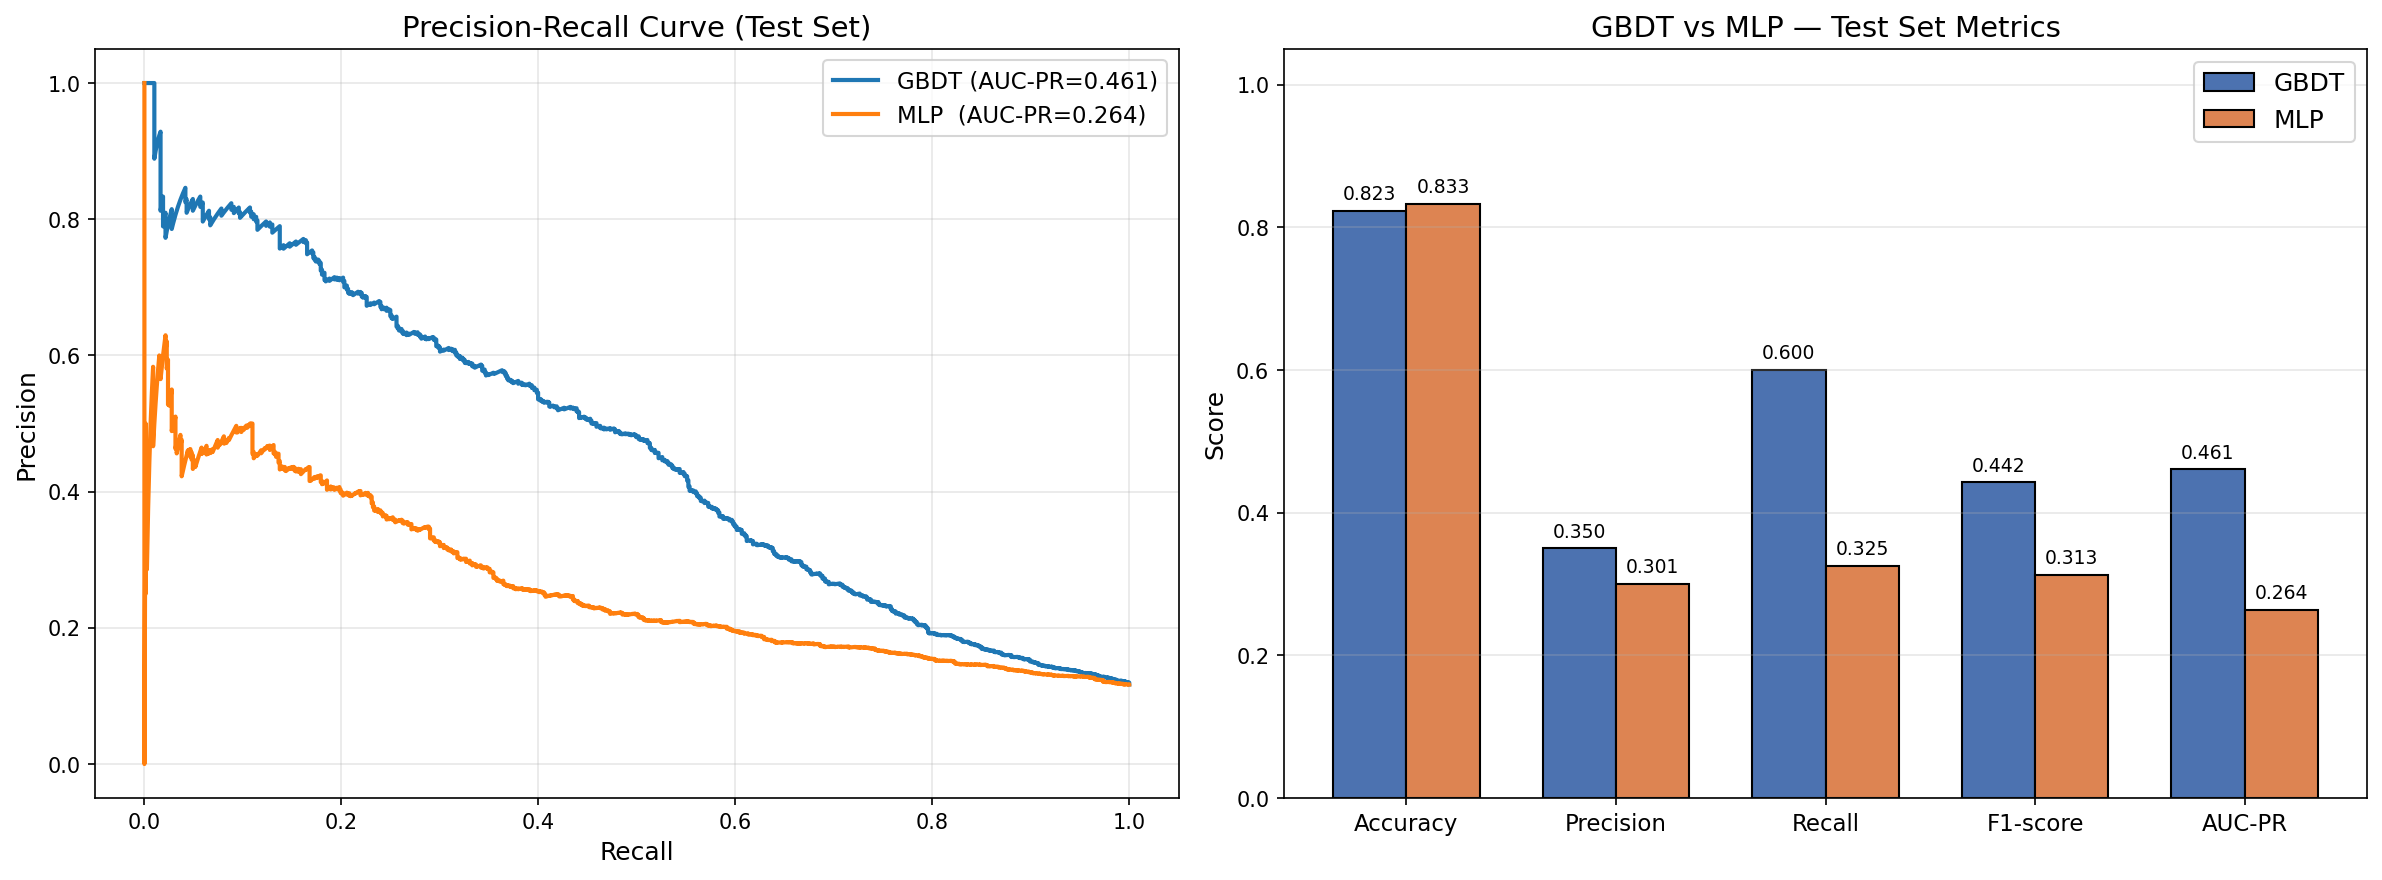
\includegraphics[width=0.75\textwidth]{fig_comparison.png}
    \caption{Left: Precision--Recall curves on the test set. GBDT dominates
             across all recall levels. Right: side-by-side bar chart of key
             metrics.}
    \label{fig:comparison}
\end{figure}

\subsection{When to prefer GBDT vs.\ MLP}

GBDT excels on \textbf{structured, tabular data} with mixed feature types,
class imbalance, and interpretability requirements. It requires minimal
preprocessing, trains extremely fast, and has built-in regularization. MLP may
be preferred for very large datasets with complex non-linear interactions among
continuous features, or for inherently high-dimensional inputs (embeddings,
images, time-series). For this medium-sized tabular dataset with categoricals
and imbalance, GBDT is the clear winner.

\subsection{Interpretability}

GBDT provides \textbf{built-in feature importance} (Figure~\ref{fig:xgb_importance}).
We identified previous campaign outcome, contact method, campaign month, and
account balance as top predictors---directly actionable for the bank's marketing
strategy. MLP is a black box: the learned weights across multiple hidden layers
do not map to intuitive, feature-level explanations. Post-hoc techniques (SHAP,
permutation importance) can approximate interpretability but add complexity and
are not inherent to the model.

\subsection{Handling categoricals and missing values}

XGBoost handles missing values \textbf{natively} by learning optimal split
directions for absent data. It also works well with encoded categoricals since
tree splits impose no ordinal assumptions. MLP requires all features to be
numeric and standardized---categoricals must be one-hot encoded and missing
values imputed \emph{before} training, making the pipeline more complex and
introducing additional design choices.

\subsection{Sensitivity to hyperparameters}

MLP proved \textbf{significantly more sensitive}. Our experiments showed:
\begin{itemize}[nosep]
    \item F1 ranged from 0.31 to 0.41 across learning rates and activations.
    \item Without class balancing, recall for ``Yes'' was only 0.24---the model
          simply did not learn the minority class.
    \item Deeper architectures \emph{hurt} F1 despite lowering training loss.
\end{itemize}
GBDT was robust: the baseline with near-default parameters already achieved
F1\,$=$\,0.45, and tuning provided only marginal improvement. GBDT's built-in
regularization (\texttt{max\_depth}, \texttt{subsample}, \texttt{reg\_lambda})
makes it naturally resistant to overfitting without careful manual tuning.

% =========================================================================
\section{Discussion}
% =========================================================================

\subsection{Bias--Variance Reflection}

GBDT reduces bias via \textbf{sequential boosting} (each tree corrects prior
errors) and controls variance through regularization (depth limits, subsampling,
L1/L2 penalties)---well-suited to medium-sized tabular data.
MLP reduces bias via \textbf{flexible function approximation} but is prone to
high variance with limited data. Oversampling addressed class imbalance but
introduced variance through duplicated samples, reflected in the inflated CV
F1 (0.93 on balanced data) vs.\ test F1 (0.31 on real data).

\subsection{Key lessons learned}

\begin{enumerate}[nosep]
    \item \textbf{Class imbalance must be handled explicitly.}
          \texttt{scale\_pos\_weight} worked cleanly for GBDT; MLP required
          oversampling, adding complexity and inflating CV scores.
    \item \textbf{Accuracy is misleading under imbalance.} MLP's higher
          accuracy (83.3\% vs.\ 82.3\%) was due to more aggressive ``No''
          predictions. F1 and AUC-PR are more informative.
    \item \textbf{Simpler MLP architectures can outperform deeper ones.}
          Extra capacity was used to predict the majority class more
          confidently, \emph{decreasing} F1.
    \item \textbf{Feature scaling is non-negotiable for neural networks.}
          Trees are invariant to feature scale.
\end{enumerate}

\subsection{Limitations}

\begin{itemize}[nosep]
    \item \textbf{Duration removed:} including it would dramatically improve
          both models but at the cost of realism.
    \item \textbf{Oversampling artifacts:} random oversampling with replacement
          can cause overfitting. SMOTE or class-weighted loss functions (e.g.,
          via PyTorch) could be explored as alternatives.
    \item \textbf{MLP framework:} scikit-learn's \texttt{MLPClassifier} lacks
          modern regularization (dropout, batch normalization, learning rate
          scheduling). A PyTorch implementation could close the performance
          gap with GBDT.
    \item \textbf{Feature engineering:} only basic derived features were
          created. Interaction terms and campaign timing patterns could improve
          both models.
\end{itemize}

% =========================================================================
\section{AI Tool Disclosure}
% =========================================================================

\begin{itemize}[nosep]
    \item \textbf{Tool used:} Claude (Anthropic), via Claude Code CLI.
\end{itemize}

\paragraph{What it contributed:}
\begin{itemize}[nosep]
    \item Generating the majority of the code for data loading, cleaning,
          model training, hyperparameter tuning, and evaluation.
    \item Suggesting different preprocessing options (e.g., how to handle
          ``unknown'' values, whether to keep or drop the \texttt{duration}
          column, which encoding strategy to use for categoricals).
    \item Implementing class imbalance handling (oversampling for MLP,
          \texttt{scale\_pos\_weight} for XGBoost) and explaining trade-offs.
    \item Drafting the \LaTeX\ report structure and text based on my guidance.
\end{itemize}

\paragraph{My own contributions:}
\begin{itemize}[nosep]
    \item Preparing the workspace: downloading and extracting the dataset,
          creating the Python notebook, and selecting the 17-feature dataset
          version.
    \item Making all modeling decisions: choosing to keep ``unknown'' as its
          own category, dropping \texttt{duration} for realism, selecting
          one-hot encoding over label encoding, and deciding on feature
          engineering choices.
    \item Reviewing, running, and verifying all code and outputs cell by cell.
    \item Reviewing and understanding training and evaluation results---such as
          identifying the MLP validation score plateau, noticing the
          deeper-networks-hurt-F1 pattern, and questioning the flat
          validation curve.
    \item Instructing Claude on what to discuss in each section of the report
          and requesting specific adjustments to content and formatting.
\end{itemize}

\end{document}
